% !TeX root = ../main.tex

\chapter{空間與位置}
\label{ch:space}

前一章曾提到過,學會控制空間就學會排版了!Knuth\index{Knuth} 教授在他的 \textit{The \TeX{}book}\index{The TeXbook@\textit{The \TeX{}book}} 一書中也曾形容使用 \TeX{} 排版的情形:一個版面就像一個含有膠水(glue\index{glue})的頁面,然後每一個要排版的內容就是各種不同的 box\index{box},在這些 box 還沒有固定正確位置時,都是可以移動的(膠水還沒有乾),一旦排版完成,膠水就乾了,於是每個 box 的位置就固定無法再移動了,除非又從頭再來。

一個字母、一個單字、一個句子、一個段落、一個符號、一個圖形、一個表格都可能構成一個 \TeX{} 的 box,甚至 box 中還有 box 的情形。這章想討論的,就是這個 box 如何安置他們到正確的位置,讓每個 box 之間的空間都能達到恰到好處,所以,到底是在控制 boxes 的屬性、位置,還是調整 glue 的空間,就看各位怎麼去看待了(請注意,box 不一定是可見的!在 \TeX{} 裡頭,glue 是可以調整的。)。

我們前面所討論到的英文句點後空白的調整、italic correction\index{italic correction}、\verb|\linespread|\index{linespread@\verb=\linespread=} 及 \verb|\parindent|\index{parindent@\verb=parindent=} 這些都是在調整 glue。通常,在 \LaTeX{} 系統裡頭,指定單位常常不會是絕對固定的,會視情形做小限度的自動微調,這是版面空間配置上的需要。

\section{\LaTeX{} 中使用的度量單位}
\label{sec:units}

要精確描述和調整 \LaTeX{} 中的空間及位置,我們必需要有個標準的度量單位。以下都是在 \LaTeX{} 常會用到的單位。這裡有絕對單位及相對單位之分,除非必要,不然,一般是建議使用相對單位,原因是,他會隨著文稿字型大小改變時跟著做適當的調整。當然,在很講求精確、固定大小的顯示時,就得使用絕對單位了。

這裡如果是閱覽 HTML 格式版本,請另參考 PDF 格式版本,以免表示上失真。以下表格中所畫出來的長度僅供參考用。

\subsection{絕對單位}
\index{絕對單位}

\begin{quote}
   \begin{tabular}{>{\tt}lll}
      單位名稱 & 意義                         & 長度            \\
      \hline
      pt       & point, $1/72.27$~inch        & \drawwidth{1pt} \\
      bp       & Adobe big point, $1/72$~inch & \drawwidth{1bp} \\
      pc       & pica, 12pt                   & \drawwidth{1pc} \\
      mm       & millimeter, $1/25.4$~inch    & \drawwidth{1mm} \\
      cm       & centimeter, 10mm             & \drawwidth{1cm} \\
      in       & inch, 25.4mm                 & \drawwidth{1in} \\
   \end{tabular}
\end{quote}

這裡要注意的是 \TeX{}/\LaTeX{} 系統中所謂的點(point)\index{點(point)},指的是一般的 printer point\index{printer point},也就是 $1/72.27$~inch,但在 Adobe 的規格中,例如 \textsc{PostScript}\index{PostScript@\textsc{PostScript}} 語言中的所謂點,他是 big point\index{big point},等於 $1/72$~inch(小數點的部份捨去了),會比一般的 print point 稍微大一點點。

\subsection{相對單位}
\index{相對單位}

\begin{quote}
   \begin{tabular}{>{\ttfamily}lll}
      單位名稱 & 意義                        & 長度            \\
      \hline
      em       & 約正在使用字型字母 M 的寬度 & \drawwidth{1em} \\
      ex       & 約正在使用字型字母 x 的高度 & \drawwidth{1ex} \\
   \end{tabular}
\end{quote}

在 \TeX{} 裡頭所謂的 em\index{em},其實,精確而言是指在 Knuth 教授設計的 Computer Modern 字型裡頭的 em-dash\index{em-dash} 的寬度,由於字母 M 實際上是包在字型上所謂的 em-square 假想方格中,而 em 所指的寬度是指這個 em-square\index{em-square} 的寬度,但字母 M 本身並不全佔有這個 em-square,因此這樣就會造成差異了。所以以字母 M 的寬度來說明的話容易有疑義。\LaTeX{} 有個指令 \verb|\quad|\index{quad@\verb=\quad=} 這就是產生一個正確 em 的寬度的空白,所以在 Knuth 教授的 \textit{The \TeX{}book} 中,說明 em 就直接說他是一個 `quad' 的寬度。

\section{版面大小}
\label{sec:layout}\index{版面大小}

我們對於所能控制的一整張紙的範圍都可以稱為版面。當然,我們的內文(body)\index{內文(body)}並不是佔滿整張紙的範圍,上下左右都會留有一定的空白。小時候在宣紙上練習寫毛筆,老一輩的都會要我們留「天地」,這就是指內文四周的空白,除了視覺上的理由,大概也是人生的哲理吧?:-)

在編輯上,也有人稱內文(body)的部份為「版心」或「版口」\index{版心}\index{版口},四周的空白部份,則稱為「版邊」\index{版邊}。突破版心、版邊的設計,就稱之為「出血」\index{出血},例如,以背景圖佈滿整張紙當做是背景的場合,以這個背景圖而言,就無所謂版邊了。但這在 \LaTeX{} 通常是不會有這種情況出現,除非特意去指定內文和紙張大小同樣範圍。

當然,在內文以外的空白,也並非全是空白,他包含了頁足(footer)\index{頁足(footer)},頁眉(header)\index{頁眉(header)}及邊註(marginal note)\index{邊註}\index{marginal note}的部份,記載關於頁數、註解等資訊。

\subsection{版面圖解}
\label{subsec:layout}

\begin{quote}
   \begin{center}
      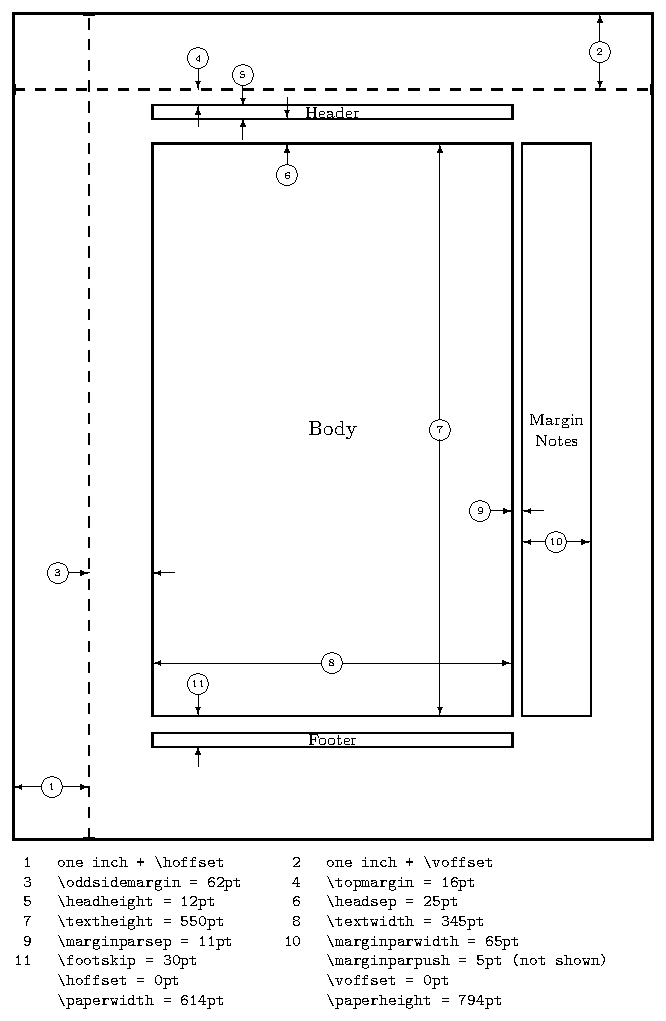
\includegraphics{layout-r}
   \end{center}
\end{quote}

這裡所謂的紙張大小\index{紙張大小},指的是 {\ttfamily paperwidth}\index{paperwidth} 和 {\ttfamily paperheight}\index{paperheight} 所圍成的範圍,並非實際上手上拿到的紙張大小,實際在手上的紙張通常會略大於我們這裡的所謂紙張,所以,正式列印時,還需做微調或截切才會是真正的這裡所謂的紙張大小(版面大小\index{版面大小})。

這是 10pt 內文大小,如果不指定紙張的話,\LaTeX{} 預設會使用美式 {\ttfamily letterpaper}\index{letterpaper} 的大小,如要使用歐、日式的 {\ttfamily a4paper}\index{a4paper} 的話,要另行指定。我們可以稍微看一下 \LaTeX{} 預設是如何安排版面空間的。其中 Header(頁眉)、Footer(頁足)及邊註的空間是不含括在內文 Body 裡頭的,這裡是只是單面的圖,如果是雙面的話,那偶數頁和奇數頁的邊註是要左右對換的,也就是說這個圖是奇數頁,偶數頁的話,邊註是在左邊。

這裡我們來看一下這些值所代表的意義:

\begin{quote}
   \begin{tabular}{ll}
      指令(值)              & 意義                         \\
      \hline
      \verb=\paperwidth=  & 紙張的寬度                   \\
      \verb=\paperheight=  & 紙張的高度                   \\
      \verb=\textwidth=  & 內文(body)的寬度           \\
      \verb=\textheight= & 內文(body)的高度           \\
      \verb=\headheight= & 頁眉(header)長度           \\
      \verb=\headsep= & 頁眉與內文間的距離           \\
      \verb=\footskip= & 內文底至頁足底之距離         \\
      \verb=\topmargin= & 頁眉上方的空白               \\
      \verb=\marginparwidth= & 邊註的寬度                   \\
      \verb=\marginparsep= & 邊註與內文的距離             \\
      \verb=\marginparpush= & 兩邊註間距                   \\
      \verb=\oddsidemargin= & 內文左邊的空白大小           \\
      \verb=\hoffset= & 微調版面在實際紙張的左右位置 \\
      \verb=\voffset= & 微調版面在實際紙張的上下位置 \\
      \index{paperwidth@\verb=\paperwidth=}\index{paperheight@\verb=\paperheight=}%
      \index{textwidth@\verb=\textwidth=}\index{textheight@\verb=\textheight=}%
      \index{headheight@\verb=\headheight=}\index{headsep@\verb=\headsep=}%
      \index{footskip@\verb=\footskip=}\index{topmargin@\verb=\topmargin=}%
      \index{marginparwidth@\verb=\marginparwidth=}\index{marginparsep@\verb=\marginparsep=}%
      \index{marginparpush@\verb=\marginparpush=}%
      \index{oddsidemargin@\verb=\oddsidemargin=}%
      \index{hoffset@\verb=\hoffset=}\index{voffset@\verb=\voffset=}%
   \end{tabular}
\end{quote}

\verb|\hoffset| 及 \verb|\voffset| 就是在調整版面在實際紙張上的正確位置,這樣印出來的時候才會在實際紙張的中央。

頭昏了嗎?這很正常,因為 \LaTeX{} 的版面設定對初接觸的人來說,是惡名昭彰的困難、麻煩,因此這裡不多談他的設定,剛開始實在沒有必要把時間花在這個地方。如果實際想調整版面,建議使用 {\sffamily geometry}\index{geometry@\textsf{geometry}} package。舉個例子,想讓各邊緣是 2cm 就好,那只要在 preamble\index{preamble} 區設定:

\begin{quote}
   \begin{verbatim}
\usepackage[margin=2cm]{geometry}
\end{verbatim}
\end{quote}

就可以了,如果以 12pt 大小的字,{\ttfamily a4paper} 紙張大小的設定的話,以中文而言,大約是每行 40 個中文字,這是內文的寬度。可以視情形自行調整 {\ttfamily margin}\index{margin} 的值就行了。我們很希望,下一版的 \LaTeX{} 能對這方面做改善,以方便使用者設定。
%更精確、詳細的設定方法,我們留到後面說明書籍成書時再來談,這樣就不致影響我們學習的正常進度。

\subsection{紙張大小}

\begin{quote}
   \begin{tabular}{>{\ttfamily}ll>{\ttfamily }ll}
      紙張    & 大小      & 紙張           & 大小        \\
      \hline
      a4paper & 21x29.7cm & letterpaper    & 8.5x11in    \\
      a5paper & 14.8x21cm & legalpaper     & 8.5x14in    \\
      b5paper & 17.6x25cm & executivepaper & 7.25x10.5in \\
   \end{tabular}
\end{quote}

至於如何指定紙張大小,這裡先簡單說明一下這篇文章的設定,談到 \LaTeX{} 的文稿類別時會再詳細說明。

\begin{quote}
   \begin{verbatim}
% 本文的設類別設定
\documentclass[12pt,a4paper]{report}
\end{verbatim}
\end{quote}

所以,這篇文章使用的是 {\ttfamily a4paper},內文字型的大小是 12pt。方括號的參數是選項,可以省略,如果省略的話,預設值就是 10pt/{\ttfamily letterpaper}。

\section{調整橫向空間}

這裡的橫向空間,例如 \verb|~|\index{~@\verb=~=} 這單字間正常空白,及 \verb|\quad| 這個 em\index{em} 寬度空白,都是在調整橫向的空白。但如果是要更大、或更小的空白時該如何調整呢?底下我們就來看看 \LaTeX{} 中有什麼控制指令可以運用:

\subsection{調整橫向空間的指令}

\begin{quote}
   \begin{tabular}{ll}
      指令                    & 意義                                                    \\
      \hline
      \verb=\hspace{單位}= & 向右空出某個度量單位的空白,如果是負數,則是向左        \\
      \verb=\hfill= & 讓左右兩旁的文字往兩邊擴張至一個行寬為止                \\
      \verb=\quad= & 空出一個 em 單位的空白                                  \\
      \verb=\qquad= & 空出二個 em 單位的空白                                  \\
      \verb=\thinspace= & 空出 $1/12$ 個 em 單位的空白                            \\
      \verb=\enspace= & 空出 $1/2$ 個 em 單位的空白                             \\
      \verb=\dotfill= & 作用和 \verb|\hfill| 相同,只是空白變成點     \\
      \verb=\hrulefill= & 作用和 \verb|\hfill| 相同,只是空白變成一橫線 \\
      \verb=\centering= & 此指令以後的文字將會居中排列,左右沿將不切齊            \\
      \verb=\raggedright= & 此指令以後的文字將會居左排列,右沿將不切齊              \\
      \verb=\raggedleft= & 此指令以後的文字將會居右排列,左沿將不切齊              \\
      \verb=\centerline{}= & 將大括號內的文字居中排列
   \end{tabular}
\end{quote}
\index{hspace@\verb=\hspace=}\index{hfill@\verb=\hfill=}%
\index{quad@\verb=\quad=}\index{qquad@\verb=\qquad=}%
\index{thinspace@\verb=\thinspace=}\index{enspace@\verb=\enspace=}%
\index{dotfill@\verb=\dotfill=}\index{hrulefill@\verb=\hrulefill=}%
\index{centering@\verb=\centering=}\index{raggedright@\verb=\raggedright=}%
\index{raggedleft@\verb=\raggedleft=}\index{centerline@\verb=\centerline{}=}

一行的行首使用 \verb|\hspace{單位}| 時將會失效,這時可以加個星號,例如 \verb|\hspace*{3em}|。

在使用 \verb|\centerline{}| 的場合,對於短文句很方便,因為他不會影響以下的文字,但他也不會折行,甚至加入換行符號也無效。所以如果文句長度超過一行的行寬,他會超出邊界,甚至就首尾的文字就看不到了。

其中 \verb|\thinspace| 又可以使用簡化的 \verb|\,| 來代替,主要是用在引號中又有引號的情形,通常這種情形,兩引號之間要有個間隔,以便區分,例如:

\begin{quote}
   \begin{verbatim}
``\,`Superman', he said.''
\end{verbatim}
\end{quote}

表現出來會是:

\begin{quote}
   ``\,`Superman', he said.''
\end{quote}

這樣才能區分出不同引號,否則會變成一個連三個 grave accent\index{grave accent} 的引號。請注意,由於這個指令是由非字母符號構成,所以,他的作用範圍在遇到符號本身後就結束了,後面不必空白或以大括號來限制其作用範圍,就好像曾提到過的 \verb|\@| 一樣的情形。

\subsection{調整橫向空間的環境}

\begin{quote}
   \begin{tabular}{ll}
      \verb|\begin{center}...\end{center}| & 讓這個環境內的內容置中               \\
      \verb|\begin{flushleft}...\end{flushleft}| & 讓這個環境內的內容靠左               \\
      \verb|\begin{flushright}...\end{flushright}| & 讓這個環境內的內容靠右               \\
      \verb|\begin{raggedright}...\end{raggedright}| & 讓這個環境內的內容靠左,右沿將不切齊 \\
      \verb|\begin{raggedleft}...\end{raggedleft}| & 讓這個環境內的內容靠右,左沿將不切齊 \\
   \end{tabular}
\end{quote}
\index{center@\texttt{center}}\index{flushleft@\texttt{flushleft}}%
\index{flushright@\texttt{flushright}}\index{raggedright@\texttt{raggedright}}%
\index{raggedleft@\texttt{raggedleft}}

進入環境,和上一節提到的指令,兩者有什麼不同呢?最大的不同是,這可以方便的指定一個範圍的文句讓他作用,而不會影響環境以外的文句。其次,進入環境,縱使和上下行連在一起,沒有空出空白行,他也會自動的在上、下行空出個空白行出來,使用指令的話則不會。

咦!這裡怎麼又有個 {\ttfamily raggedright} 及 {\ttfamily raggedleft}?原來他也是可以當環境來使用。由於這兩個指令會使以下的內容的左、右沿不切齊,因此使用上要非常小心,除非本來就想讓內文的左、右沿不切齊,否則,最好是使用有範圍限制的方式。當然,如果這兩個指令是用在某個其他環境範圍內,他的作用也將僅限於這個環境內,不會影響這個環境外的文句。

\subsection{引文環境}
\index{引文環境}

引文通常就是引用他人的文句,在引文的段落,兩旁都會出現內縮的情形,以便和正文相區隔,這也是一種空間的配置,可增加文章的易讀性。在 \LaTeX{} 裡頭有三種引文環境:{\ttfamily quote}, {\ttfamily quotation}, {\ttfamily verse}。這三者看起來很像,但有些微的差異。

\begin{quote}
   \begin{tabular}{>{\ttfamily }lll}
      環境      & 適用時機         & 特性                                     \\
      \hline
      quote     & 較短的短引文     & 每個段落第一行不內縮                     \\
      quotation & 多個段落的長引文 & 每個段落第一行會內縮                     \\
      verse     & 詩歌、詞引文     & 每個段落的第一行不內縮,但第二行起會內縮 \\
   \end{tabular}
\end{quote}
\index{quote@\texttt{quote}}\index{quotation@\texttt{quotation}}%
\index{verse@\texttt{verse}}

在 {\ttfamily verse} 的情形,通常會使用 \verb=\\=\index{\\@\verb=\\=} 來換行以便控制每一行的寬度。而且段落間距\index{段落間距}將不受外在設定的影響,其中 {\ttfamily quote} 和 {\ttfamily verse} 環境會預插入適當的段落間距,而 {\ttfamily quotation} 環境則不會。

底下我們來看看調整橫向空間的一個綜合實例:

\begin{quote}
   \begin{verbatim}
% example11.tex
\documentclass{article}
\usepackage{CJK}
\begin{document}
\begin{CJK}{Bg5}{hwmm}
\section{hspace}
\hspace*{2em}這是一個橫向空間調整的測試。\\
這是一個\hspace{2em}橫向空間調整的測試。\\
這是一個 \hspace{2em} 橫向空間調整的測試。
\section{hfill}
這是一個\hfill{}橫向空間調整的測試。
\section{quad}
這是一個\quad{}橫向空間調整的測試。\\
這是一個 \quad{} 橫向空間調整的測試。\\
這是一個\qquad{}橫向空間調整的測試。
\section{dotfill}
這是一個\dotfill{}橫向空間調整的測試。\\
這是一個 \dotfill{} 橫向空間調整的測試。
\section{hrulefill}
這是一個\hrulefill{}橫向空間調整的測試。
\section{center}
\begin{center}
這是一個橫向空間調整的測試。
\end{center}
\section{flushleft}
\begin{flushleft}
這是一個橫向空間調整的測試。
\end{flushleft}
\section{flushright}
\begin{flushright}
這是一個橫向空間調整的測試。
\end{flushright}
\section{quote}
這是節錄自伊索寓言的節錄故事:
\begin{quote}
An antwent to the bank of a river to quench its thirst, and
being carried away by the rush of the stream, was on the
point of drowning.
A Dove sitting on a tree overhanging the water plucked a
leaf and let it fall into the stream close to her. The Ant
climbed onto it and floated in safety to the bank.
\end{quote}
\section{quotation}
這是節錄自伊索寓言的節錄故事:
\begin{quotation}
An antwent to the bank of a river to quench its thirst, and
being carried away by the rush of the stream, was on the
point of drowning.
A Dove sitting on a tree overhanging the water plucked a
leaf and let it fall into the stream close to her. The Ant
climbed onto it and floated in safety to the bank.
\end{quotation}
\section{verse}
這是節錄自伊索寓言的節錄故事,這是節錄自伊索寓言的節錄故事,%
這是節錄自伊索寓言的節錄故事,這是節錄自伊索寓言的節錄故事:
\begin{verse}
An antwent to the bank of a river to quench its thirst, and
being carried away by the rush of the stream, was on the
point of drowning.
A Dove sitting on a tree overhanging the water plucked a
leaf and let it fall into the stream close to her. The Ant
climbed onto it and floated in safety to the bank.
\end{verse}
\section{centering}
\centering
這是一個橫向空間調整的測試。\\ % 這裡要換行,否則會是 \raggedright 的作用
\raggedright
\section{centerline}
\centerline{這是一個橫向空間調整的測試。}
\section{raggedright}
\raggedright
這是一個橫向空間調整的測試。
\section{raggedleft}
\raggedleft
這是一個橫向空間調整的測試。
\end{CJK}
\end{document}
\end{verbatim}
\end{quote}

編譯好的結果如下:

\begin{quote}
   \url{http://edt1023.sayya.org/tex/latex123/example11.tex}\\
   \url{http://edt1023.sayya.org/tex/latex123/example11.pdf}
\end{quote}

要注意是指令前後的空白,像 \verb|\hspace|, \verb|\dotfill|, \verb|\hrulell| 這類指令,指令前後空白都會算進去的。\verb|\quad|, \verb|\qquad| 這類指令,則後面的空白也是會算入的。另外,由例子中可以看出來,一個 em\index{em} 的寬度,大約是一個中文字的寬度,所以,我們預設使用 10pt 的字,這個 em 寬度就相當於 10pt 的寬度,所以,我們在第一行插入了 2em 寬度的空白,也就好像是內縮了兩個中文字一樣。

\section{調整縱向空間}

\begin{quote}
   \begin{tabular}{ll}
      \verb=\vspace{單位}=      & 向下空出某個單位的空白(行),負數則是向上                      \\
      \verb=\bigskip=      & 產生 12pt(11--12pt)的垂直空白(行)                           \\
      \verb=\medskip=      & 產生 6pt(5--7pt)的垂直空白(行)                              \\
      \verb=\smallskip=      & 產生 3pt(2--4pt)的垂直空白(行)                              \\
      \verb=\vfill=      & 和 \verb|\hfill| 類似,作用是將某段落向上頂,或往下擠 \\
      \verb=\parskip=單位= & 調整全文每個段落間的距離為某個單位
      \index{vspace@\verb=\vspace=}\index{bigskip@\verb=\bigskip=}%
      \index{medskip@\verb=\smallskip=}\index{vfill@\verb=\vfill=}%
      \index{parskip@\verb=\parskip=}
   \end{tabular}
\end{quote}

其中的 \verb|\bigskip, \medskip, \smallskip| 並非固定的,他們會視上下文脈絡的需要自動做微調,以達到一整頁較一致的空間配置。\verb|\vspace| 如果是出現在一頁的第一行或最後一行時,將會失去作用,這時可以加個星號,\verb=\vspace*{單位}=\index{vspace@\verb=\vspace*=}。

為了維持版面的一致性\index{版面一致性},使用縱向空間調整的指令時要特別留意,例如章節標題上下的空間、各段落間的空間,進入環境前後所空出的空間,這都有一個固定值,\LaTeX{} 會自動去調整,不必由使用者自行動手,除非是封面這種單獨頁。所以,使用縱向空間調整指令時,要非常注意整體的一致性,這也是排版上的一個很重要的原則。

這裡舉這篇文章的內頁封面\index{內頁封面}為例來綜合說明,橫、縱向空間的運用。還記得第 \ref{sec:titlepage} 節的 title page\index{title page} 的指令嗎?其實我們也可以自行設計一個獨立的內頁封面,使用的是 \LaTeX{} 本身的 {\ttfamily titlepage}\index{titlepage@\texttt{titlepage}} 環境。這裡的圖檔引用是我們還沒有學習到的,沒關係,只要大原則抓住就行了。

\begin{quote}
   \begin{verbatim}
% example12.tex
\documentclass[12pt,a4paper]{report}
\usepackage{CJK}     % 引入所需要的 packages
\usepackage{graphicx}
\begin{document}
\begin{CJK}{Bg5}{hwmm}
\begin{titlepage}    % 使用 titlepage 環境
\vspace*{5ex}
  \begin{flushright} % 大標題靠右
    \Huge\textbf{大家來學 \LaTeX}
  \end{flushright}
  \rule{\textwidth}{.256ex}
  \begin{flushleft}  % 版本號碼及日期靠左,和大標題之間以一橫線隔開
    Version 0.1 draft\\
    \today
  \end{flushleft}    % 圖檔位於中央偏左
  \vspace{8ex}       % 空出 8ex 的垂直空間
  \hspace{2em}\includegraphics[scale=.75]{cover2.1} % 引入圖檔,並將這個
  \vspace{8ex}                                      % 圖檔橫向右移 2em
  \begin{flushright} % 作者資訊靠右
    By Edward G.J. Lee 李果正\\
    Email:\texttt{edt1023@info.sayya.org}
  \end{flushright}
\end{titlepage}
\end{CJK}
\end{document}
\end{verbatim}
\end{quote}

由於配合版面的問題,其中有一些數據有更動,而且也省略了一些我們還沒有學習到的 packages,但大結構則和原始文稿一樣。所以,和這篇文章的 PDF 格式比較會發現,大標題的字體小了一點,而且沒有顏色,也沒有超連結\index{超連結}。

使用 {\ttfamily titlepage}\index{titlepage@\texttt{titlepage}} 環境後,在 {\ttfamily report/book}\index{report@\texttt{report}}\index{book@\texttt{book}} 文稿他會自成一沒有頁數的單獨頁,在 {\ttfamily article}\index{article@\texttt{article}} 類別,因為會和內文連接,所以,在選項的部份要多加一個 {\ttfamily titlepage}\index{titlepage} 的選項。另外,在 {\ttfamily titlepage} 裡頭就不能再使用 \verb|\title|\index{title@\verb=\title=}, \verb=\author=\index{author@\verb=\author=} 指令了,在本文的地方也不必再下 \verb=\maketitle=\index{maketitle@\verb=\maketitle=} 指令。

編譯好的例子如下:

\begin{quote}
   \url{http://edt1023.sayya.org/tex/latex123/example12.tex}\\
   \url{http://edt1023.sayya.org/tex/latex123/example12.pdf}
\end{quote}

這裡要特別說明的是,引入圖檔要使用 \textsf{graphicx}\index{graphicx@\textsf{graphicx}} package(這是最常用的,也有其他的方法來引用),引入的指令是 \verb=\includegraphics=\index{includegraphics@\verb=\includegraphics=},這個我們會在第 \ref{ch:graphic} 章會討論,在這裡我們把圖檔縮小成為原圖的 {\ttfamily 75\%},否則整個封面會超出一頁。這個圖檔是由 \MP\index{metapost@\MP} 檔案所編譯而來的,他是一種 eps 圖檔\index{eps 圖檔}(簡單的說,是含有邊界數據去除不必要周圍空白的 ps 檔\index{ps 檔},方便引入或輸出至文稿中),編譯的方法如下:

\begin{quote}
   \begin{verbatim}
mpost cover2.mp
\end{verbatim}
\end{quote}

這樣就會產生 {\ttfamily cover2.1} 這個 eps 圖檔,這樣就可以直接引入了。他的原始碼及 eps 圖檔在:

\begin{quote}
   \url{http://edt1023.sayya.org/tex/latex123/cover2.mp}\\
   \url{http://edt1023.sayya.org/tex/latex123/cover2.1}
\end{quote}


\section{條列環境}

條列環境\index{條列環境}也是屬於一種空間的控制,他把一些文字按一定的方式來排列,條列環境中一些起頭的符號、文數字或字串,我們稱之為項目標籤(item label)\index{項目標籤(item label)},利用這些不一樣的排列位置及不一樣的項目標籤起頭來敘述文句,就可以達到醒目的作用。這是以章節分隔以外,相當常用讓內容一目了然的方法,建議多多利用。請千萬記得,環境中還可以有環境,而且以下三種的條列方式可以混合交叉使用。

\subsection{項目式條列環境(itemize)}
\index{項目式條列環境(itemize)}

這是以符號來起頭醒目的一種條列方式。例如:

\begin{quote}
   \begin{verbatim}
\begin{itemize}
\item 第一大項,這裡是第一大項。
\item 第二大項,這裡是第二大項。
 \begin{itemize}
 \item 第一小項,這裡是第一小項。
 \item 第二小項,這裡是第二小項。
 \end{itemize}
\item 第三大項,這裡是第三大項。
\item 第四大項,這裡是第四大項。
\end{itemize}
\end{verbatim}
\end{quote}

排版出來會變成:

\begin{quote}
   \begin{itemize}
      \item 第一大項,這裡是第一大項。
      \item 第二大項,這裡是第二大項。
            \begin{itemize}
               \item 第一小項,這裡是第一小項。
               \item 第二小項,這裡是第二小項。
            \end{itemize}
      \item 第三大項,這裡是第三大項。
      \item 第四大項,這裡是第四大項。
   \end{itemize}
\end{quote}

\subsection{列舉式條列環境(enumerate)}
\label{subsec:enume}\index{列舉式條列環境(enumerate)}

這是以數目字或字母或羅馬數字來起頭醒目的條列方式。同樣的例子,改成 {\ttfamily enumerate} 的話,會排版成:

\begin{quote}
   \begin{enumerate}
      \item 第一大項,這裡是第一大項。
      \item 第二大項,這裡是第二大項。
            \begin{enumerate}
               \item 第一小項,這裡是第一小項。
               \item 第二小項,這裡是第二小項。
            \end{enumerate}
      \item 第三大項,這裡是第三大項。
      \item 第四大項,這裡是第四大項。
   \end{enumerate}
\end{quote}

\subsection{敘述式條列環境(description)}
\index{敘述式條列環境(description)}

這是以一個簡短文字敘述來起頭醒目的條列方式。再把他改成 {\ttfamily description} 的話,他是以粗體文字來起頭醒目的,這些文字要用方括號括住。

\begin{quote}
   \begin{verbatim}
\begin{description}
\item[第一大項] 這裡是第一大項。
\item[第二大項] 這裡是第二大項。
  \begin{description}
  \item[第一小項] 這裡是第一小項。
  \item[第二小項] 這裡是第二小項。
  \end{description}
\item[第三大項] 這裡是第三大項。
\item[第四大項] 這裡是第四大項。
\end{description}
\end{verbatim}
\end{quote}

排版出來的結果是:

\begin{quote}
   \begin{description}
      \item[第一大項] 這裡是第一大項。
      \item[第二大項] 這裡是第二大項。
            \begin{description}
               \item[第一小項] 這裡是第一小項。
               \item[第二小項] 這裡是第二小項。
            \end{description}
      \item[第三大項] 這裡是第三大項。
      \item[第四大項] 這裡是第四大項。
   \end{description}
\end{quote}

要注意的是,不管哪一種的條列環境,每個項目(item)的文字敘述會自動折行,這相當方便,使用者只要把條列的結構弄妥,專心打每個項目的內容就成了。而且,如果使用方括號括住一些字元、字串或符號,那帶頭的標示將會是這些字元、字串或符號,如果是列舉式的條列方式,那麼有方括號的將不被編號,會自動跳過,編號順序則會自動順延。

%\section{enumerate 巨集套件}

%\subsection{條列環境內的空間控制}


\section{線框}
\index{線框}

線框在排版上佔有一定的地位,因為他可以區隔不同的空間,也可以讓某些部份突顯出來。但是,過多的線框也是會有喧賓奪主的不好副作用,使用上可能要適可而止。這裡我們要談的是單純的線框,表格\index{表格}也是線框的一種應用,我們將會在第 \ref{ch:graphic} 章,再來談表格的處理。

%在 \LaTeX{} 的線框可分為三種:LR、Rule 及 Par。

%\begin{quote}
%\begin{tabular}
%線框種類 & 意義 \\
%\hline
%LR  & left-right,線框及線框中的內容由左至右 \\
%Rule & 
%Par
%\end{tabular}
%\end{quote}

\subsection{直線(rule)}
\index{直線(rule)}

直線也是屬於方框的一種,就是一個實體長方形,只不過,他的高或寬(線的組細)只有一點點,所以,看起來就一像直線罷了。

\begin{quote}
   \begin{verbatim}
\rule[上下位置(單位)]{寬}{高}
\end{verbatim}
\end{quote}

寬及高應不必多做解釋,那個上下位置是什麼呢?這個上下位置是和基線(baseline)\index{基線}\index{baseline}在比較的,如果沒有指定,那就是在基線的位置,如果有指定,就依正負值調整和基線的相對位置,正值由基線向上調整,負值則由基線向下調整。這裡來看個個實例就瞭解了:

\begin{quote}
   \begin{verbatim}
% example13.tex
\documentclass{article}
\parskip=3pt
\parindent=0pt
\begin{document}
This is a line.       % 畫高 1pt 寬 3cm 的橫線。
\rule{3cm}{1pt}
\rule[1ex]{3cm}{1pt}
\rule[-1ex]{3cm}{1pt}
\rule{1pt}{3cm}      % 畫高 3cm 寬 1pt 的直線。
\rule{3cm}{0pt}TEST. % 把 TEST 向右推 3cm。
\rule{2cm}{3cm}      % 畫高 3cm 寬 2cm 的實體方框。
\textcolor{blue}{This is color lines.}
\textcolor{red}{\rule{3cm}{1pt}}        % 有顏色的線框。
\textcolor{green}{\rule[1ex]{3cm}{1pt}}
\textcolor{blue}{\rule[-1ex]{3cm}{1pt}}
\end{document}
\end{verbatim}
\end{quote}

編譯好的例子在:

\begin{quote}
   \url{http://edt1023.sayya.org/tex/latex123/example13.tex}\\
   \url{http://edt1023.sayya.org/tex/latex123/example13.pdf}
\end{quote}

由例子中可以看得出來,這個畫線指令並不是單單縱、橫畫線而已,靈活運用的話,可以做出許多不同的效果,例如方條圖之類的。

\subsection{文字底線(underline)}
\index{文字底線(underline)}

有時候我們希望在書寫文字的同時,也在其下畫線。\LaTeX{} 有現成的指令可以使用,那就是 \verb|\underline{文字}|\index{underline@\verb=\underline=},會在文字底線的部份同時畫上線條。當然,使用上常常會和現在的橫線搞混,因此使用時要特別留意整個頁面上是否已經存在了許多橫線。

\subsection{方框(box)}
\index{box}

這裡主要指的文字方框,繪圖上的一般框形在第 \ref{ch:graphic} 章時再來討論。這一章的開頭就已談到,整篇文章是由一個個的 box 所構成的,這裡的方框則是一個典型的 box,他的地位,當然是和前面所說的 box 一樣,\TeX/\LaTeX{} 會把他視為一個單一的字母來處理。

我們先來看看最簡單的方框的指令:

\begin{quote}
   \begin{tabular}{ll}
      指令                     & 意義及作用                                         \\
      \hline
      \verb=\frame{文字}= & 將文字內容以可見的方框框住,方框和文字間沒有間距   \\
      \verb=\fbox{文字}= & 將文字內容以可見的方框框住,方框和文字間有一定間距 \\
      \verb=\mbox{文字}= & 作用和 \verb|\fbox| 同,但方框不可見
   \end{tabular}
\end{quote}
\index{frame@\verb=\frame=}\index{fbox@\verb=\fbox=}%
\index{mbox@\verb=\mbox=}

以上的指令都可以形成方框文字。

方框也有可以調整的指令:

\begin{quote}
   \begin{tabular}{ll}
      指令                     & 意義及作用                                             \\
      \hline
      \verb|\framebox[寬度][對齊方式]{文字}| & 與 \verb|\fbox| 同,但可指定寬度及對齊方式 \\
      \verb|\makebox[寬度][對齊方式]{文字}| & 與 \verb|\mbox| 同,但可指定寬度及對齊方式
      \index{framebox@\verb=\framebox=}\index{makebox@\verb=\makebox=}
   \end{tabular}
\end{quote}

這裡的寬度指的是方框的寬度,不指定的話,作用就如同 \verb|\fbox| 及 \verb|\mbox| 一樣,以包住整個文字範圍為寬度,由於我們不容易測知文字內容的寬度有多少,因此寬度的指定可以使用下列相對單位的方式:

\begin{quote}
   \begin{tabular}{ll}
      寬度                     & 作用                                                             \\
      \hline
      \verb|\width| & 這個寬度就是 \verb|\fbox| 圍住時的方框寬度           \\
      \verb|\height| & 這是正常基線至框頂的高度                                         \\
      \verb|\depth| & 這是正常基線至框底的高度                                         \\
      \verb|\totalheight| & 這是 \verb|\height| 和 \verb|\depth| 之總和 \\
   \end{tabular}
\end{quote}

例如,我們指定 \verb|2\width| 他的意思就是以 \verb|\fbox| 包住此文字內容時,其方框寬度的二倍寬。參數裡頭的對齊方式,可有下列幾種:

\begin{quote}
   \begin{tabular}{>{\ttfamily }ll}
      對齊方式 & 作用                                 \\
      \hline
      c        & center,文字位於方框中央,這是預設值 \\
      l        & flushleft,文字位於方框左方          \\
      r        & ushright,文字位於方框右方           \\
      s        & stretch,文字平均分分布於方框中
   \end{tabular}
\end{quote}

不指定的話,當然就是位於方框中央位置了。我們也可以指定可見方框的線的粗細,及方框和文字間的間隔距離:

\begin{quote}
   \begin{tabular}{ll}
      指令                     & 作用                 \\
      \hline
      \verb|\fboxrule=單位| & 指定方框線條粗細     \\
      \verb|\fboxsep=單位| & 指定文字和框緣的間距 %
      \index{fboxrule@\verb=\fboxrule=}\index{fboxsep@\verb=\fboxsep=}%
   \end{tabular}
\end{quote}

請注意,這不會影響 \verb|\frame{}|。如果想特別的置放方框的位置,也可以使用 \verb|\raisebox|\index{raisebox@\verb=raisebox=} 指令:

\begin{quote}
   \begin{verbatim}
\raisebox{上下位置(單位)}[深度][高度]{文字內容}
\end{verbatim}
\end{quote}

這裡的上下位置的意義和 \verb|\rule| 指令裡頭的一樣,只不過,這裡的上下位置一定要指定,沒有預設值,不指定會編譯錯誤。請千萬記得,方框中當然是還可以有方框的。我們現在就來看一個綜合的實例:

\begin{quote}
   \begin{verbatim}
% example14.tex
\documentclass{article}
\parskip=3ex
\parindent=0pt
\begin{document}
\frame{This is frame.}
\mbox{This is mbox.}
\fbox{This is fbox.}
\framebox{This is a framebox with no argumant.}
\framebox[1.5\width]{This is a framebox.}
\framebox[1.5\width][l]{This is a framebox with \texttt{l}.}
\framebox[1.5\width][r]{This is a framebox with \texttt{r}.}
\framebox[1.5\width][s]{This is a framebox with \texttt{s}.}
This is baseline.
\raisebox{3ex}[5\height]{This is a raisebox which lift 3ex.}
This is baseline.
\fbox{\raisebox{-3ex}[5\height]{This is a raisebox which lift $-$3ex.}}
\fboxrule=1.5pt
\fboxsep=8pt
\framebox[1.5\width][s]{This is a framebox with \texttt{s}.}
\end{document}
\end{verbatim}
\end{quote}

這應無需多加解釋,編譯好的例子在:

\begin{quote}
   \url{http://edt1023.sayya.org/tex/latex123/example14.tex}\\
   \url{http://edt1023.sayya.org/tex/latex123/example14.pdf}
\end{quote}

\subsection{段落方框}
\index{段落方框}

另外,也有用於段落文字的方框,可以控制某個段落出現在某特定的空間、位置。我們常常把這種安排稱為迷你版面,把版面內容置於一個不可見的方框當中,當然,這個方框和一般的 box,例如字母,仍然處於同樣的地位,\LaTeX{} 會把他當成一個字母單位來處理。

\begin{quote}
   \begin{verbatim}
\parbox[對齊方式][高度][內文位置]{寬度}{文字內容}
\begin{minipage}[對齊方式][高度][內文位置]{寬度}
  段落內容
\end{minipage}
\end{verbatim}
\end{quote}
\index{parbox@\verb=parbox=}\index{minipage@\texttt{minipage}}

這裡的第一個選擇性參數「對齊方式」:

\begin{quote}
   \begin{tabular}{>{\ttfamily }ll}
      t & top,段落方框的上沿對齊一行的基線              \\
      b & bottom,段落方框的下沿對齊一行的基線           \\
      c & center,段落方框的中央對齊一行的基線,這是預設 \\
   \end{tabular}
\end{quote}

\verb|\parbox| 指令通常用於較短的文字內容,如果是較長的段落,那使用 {\ttfamily minipage} 環境會比較方便。這些段落方框和上面所談到的一些方框最大的不同是,段落方框本就是用來排版小段落文句,因此他會和一般正常文章段落一樣的處理,例如他會自動斷行,碰到空白行也會起新段落,但各段落預設是不縮排的,而且,在安排上會比一般的段落緊湊,一些邊緣的間距會縮減成 0pt。

高度不去指定的話,那就是以整個版面經斷行處理後,整個文字段落所形成的高度。至於內文位置指的也是 \texttt{t, b, c} 這些,意思是文字段落在方框內的上下位置,當然,這要有指定方框高度時才會有意義,因此,「內文位置」和「高度」是要同時指定的,要非常注意的是,如果指定了高度,但沒有指定內文位置,則預設是等於前面使用的「對齊方式」所指定的參數。

這些參數的使用會有些煩複,但這是彈性所帶來的「必要之惡」,不必去死記,只有在第一次接觸時把他搞清楚就夠了,實際要用到時再來查他的詳細參數,常用的指令、環境,大概多查幾次就自然而然的記起來了。
